% This is "sig-alternate.tex" V2.1 April 2013
% This file should be compiled with V2.5 of "sig-alternate.cls" May 2012
%
% This example file demonstrates the use of the 'sig-alternate.cls'
% V2.5 LaTeX2e document class file. It is for those submitting
% articles to ACM Conference Proceedings WHO DO NOT WISH TO
% STRICTLY ADHERE TO THE SIGS (PUBS-BOARD-ENDORSED) STYLE.
% The 'sig-alternate.cls' file will produce a similar-looking,
% albeit, 'tighter' paper resulting in, invariably, fewer pages.
%
% ----------------------------------------------------------------------------------------------------------------
% This .tex file (and associated .cls V2.5) produces:
%       1) The Permission Statement
%       2) The Conference (location) Info information
%       3) The Copyright Line with ACM data
%       4) NO page numbers
%
% as against the acm_proc_article-sp.cls file which
% DOES NOT produce 1) thru' 3) above.
%
% Using 'sig-alternate.cls' you have control, however, from within
% the source .tex file, over both the CopyrightYear
% (defaulted to 200X) and the ACM Copyright Data
% (defaulted to X-XXXXX-XX-X/XX/XX).
% e.g.
% \CopyrightYear{2007} will cause 2007 to appear in the copyright line.
% \crdata{0-12345-67-8/90/12} will cause 0-12345-67-8/90/12 to appear in the copyright line.
%
% ---------------------------------------------------------------------------------------------------------------
% This .tex source is an example which *does* use
% the .bib file (from which the .bbl file % is produced).
% REMEMBER HOWEVER: After having produced the .bbl file,
% and prior to final submission, you *NEED* to 'insert'
% your .bbl file into your source .tex file so as to provide
% ONE 'self-contained' source file.
%
% ================= IF YOU HAVE QUESTIONS =======================
% Questions regarding the SIGS styles, SIGS policies and
% procedures, Conferences etc. should be sent to
% Adrienne Griscti (griscti@acm.org)
%
% Technical questions _only_ to
% Gerald Murray (murray@hq.acm.org)
% ===============================================================
%
% For tracking purposes - this is V2.0 - May 2012

\documentclass{sig-alternate-05-2015}

\begin{document}

\title{Scalable data cleansing based on qualitative attributes}

\numberofauthors{1}

\author{
\alignauthor
	Mika Huttunen\\
       		\affaddr{Helsinki University}
}

\date{11 March 2018}

\maketitle

\begin{abstract}
This is an example abstract...
\end{abstract}

%
% The code below should be generated by the tool at
% http://dl.acm.org/ccs.cfm
% Please copy and paste the code instead of the example below. 
%
%\begin{CCSXML}
%<ccs2012>
% <concept>
%  <concept_id>10010520.10010553.10010562</concept_id>
%  <concept_desc>Computer systems organization~Embedded systems</concept_desc>
%  <concept_significance>500</concept_significance>
% </concept>
% <concept>
%  <concept_id>10010520.10010575.10010755</concept_id>
%  <concept_desc>Computer systems organization~Redundancy</concept_desc>
%  <concept_significance>300</concept_significance>
% </concept>
%</ccs2012>  
%\end{CCSXML}

%\ccsdesc[500]{Computer systems organization~Embedded systems}
%\ccsdesc[300]{Computer systems organization~Redundancy}

\printccsdesc

\keywords{data cleansing, big data, scalability}


% 1. INTRODUCTION
\section{Introduction}

Nowadays companies are gathering large amounts of data in different ways such as via user input, and all kinds of sensors. It's also becoming easier and easier for them to use data in all kinds of decision making, analytics, and for example in automating human-involved tasks. Problems arise when the used data is \textit{dirty}, or invalid, and thus can lead into making incorrect decisions. These can sometimes cause serious issues - especially in health care and financing sides \cite{Ilyas2015}.

Humans often make data input errors via misspelling, and sensors may grab unwanted noise along the data they're designed to catch. In fact, over $25$\% of critical data in the world?s top companies is flawed \cite{Khayyat2015}. Not to mention that today, the variety of data is also large which leads into collecting data of different formats together. \textit{Data cleansing} is the solution to the above-mentioned problem. For data processors, understanding data cleansing, and the problems it tries to solve is thus naturally important. 

Data cleansing is a research field that explores ways to improve \textit{quality} of dirty data. If data isn't of high quality, it means that it has usually both \textit{schema}, and \textit{instance} level problems \cite{Rahm2000}. Another used definition for dirty data is that it doesn't meets its usage needs. A simple example of that would be such that a front developer of a service can't provide end-users a good UI because the server cannot deliver all kinds of useful data because there are faults in the way the data is stored in the database.

Figure \ref{rahm1} shows how \textit{single-source problems} with data quality can yet be divided into schema and instance level data problems. Single-source problems simply stand for such that can occur in data that is stored in a single site with possible data replication on the database side. The same problems can also arise in \textit{multi-source} systems where the data may also be scattered across several sites. Today, there is no good solution for cleaning huge amounts of data in multi-source systems although some research towards this has been made \cite{Ilyas2015} (p. $379$).

\begin{figure}
	\centering

	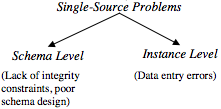
\includegraphics[scale=0.8]{figures/rahm1.png}
	\caption{Single-source data quality problems} \label{rahm1}
\end{figure}

Instance level problems in data arise as attributes of data \textit{tuples} being out of their scope, or just wrong. These contain misspellings, and \textit{outliers} by for example possible sensor errors, and processing errors before gathered data is actually stored. These problems can be detected via \textit{quantitative techniques} related to data cleansing that focus on error detection and correction based on numerical attributes of data \cite{Hellerstein2008}. If for example some framework can reduce multi-dimensional data in two-dimensional space, it's fairly easy for an expert to detect outliers in that space, and thus possible errors in the data.

Schema level problems on the other hand arise as \textit{violations} of \textit{rules} such as \textit{integrity constaints} (IC), and \textit{functional dependencies} (FD) in the data \cite{Ilyas2015} (p. $289 - 291$). As an example, functional dependency
\begin{equation}
  ZIP \rightarrow STATE \label{eq1}
\end{equation} defines a constraint between data attributes $ZIP$ and $STATE$ such that $ZIP$ implies the $STATE$. In other words, if we had a dataset with two tuples having the same $ZIP$ attribute, but different values of $STATE$, based on trusting rule \ref{eq1}, at least one of them is erroneous.

\textit{Duplicate} (or partically duplicate) data entries can also be considered both schema level, and instance level data quality problems \cite{Ilyas2015} (p. $283$). They usually appear as the same entries with some attributes having different values from each other, and thus should be classified as instance level problems. They can however be detected by similar rules that are used for other schema level problems. Consider us having a person register where each person has its name, phone number, address, zip code ($ZIP$), and state ($STATE$) defined. Now we could have two tuples with the same name, phone number, and address, but different zip codes. An error between these two tuples found be detected by rule \ref{eq1}, and could be solved either automatically, or via human interaction. 

This seminar report focuses on highly scalable \textit{qualitative} data cleansing techniques. They focus on detecting data errors in \textit{big data} via rules such as ICs, FDs, \textit{CFDs} (conditional functional dependencies), and \textit{DCs} (denial constraints). Ilays and Chu well-define the constraints in their paper \cite{Ilyas2015} (p. 287 - 301). In traditional ways, the data errors are detected by algorithms that compare data tuples trying to find violations based only on user-defined rules, or also such rules or \textit{patterns} that the data cleansing framework itself generates by processing the data. The found errors can afterwards be fixed either via totally automatic, or (partially) human guided procedures.

The rest of the report is divided as follows: in Section $2$, I will introduce recent findings related to big data cleansing, and where we stand on the field at the moment. Section $3$ gives background for following sections by introducing different kinds of techniques related to handling big data, but also for getting more accurate data cleansing results. Section $4$ discusses recent frameworks for scalable data cleansing big data, and in Section 5, I have a brief conclusion to summarise the report.

% TODO: section 5: omat ideat, algoritmit yms., conclusion: section 6


%The rest of the report is will be divided as follows. In section 2, I will summarise, where we are with big data cleansing at the moment. I'll introduce several big data cleansing techniques in more detail. The techniques can practically be divided into \textit{de-duplication} methods, \textit{sampling}, \textit{incremental cleansing}, and \textit{distributed cleansing}. I'll also discuss what kinds of problems are yet to be solved. 

% skaalautuvuus --> oletuksia, dataa usealla 'saitilla', holistic vs. non-holistic cleansing, ... ?

% In section 3, I will go through actual implementations for big data cleansing techniques. BigDansing, KATARA(?), ML frameworks, ... Section 4 discusses weak points in the papers, and in section 5, I show my own ideas to the research problem. Finally section 6 summarises the whole report. 


% Most data cleansing frameworks involve human interaction: either by training a ML classifier built-in the framework to solve conflicts on its own, or solving conflicts themselves

%Detecting, and removing (partially) duplicate entries is one of the key areas in data cleansing, and frameworks such as \textit{DeDoop} and \textit{Dis-Dedup} which is examined in section $4$ are specifically designed for their detection.

%Qualitative techniques are used to detect and correct data errors based on \textit{integrity constraints}, or \textit{patterns} in the data \cite{Ilyas2015}. In a database, an example of an integrity constraint could be such that each person should have unique social security number. A pattern on the other hand could be such that for each person, their ZIP code would define the city they live in. If we have several people with ZIP code being $00100$, and city as Helsinki, and yet another person with same ZIP code, but city being Turku, the latter mentioned person should be considered erroneous.



% 2. LITERATURE REVIEW
\section{Literature review}

- M��rittele ensin dirty / low quality data\\
- Seuraavaksi hyv� selitt��, mist� qualitative data analysisiss� ja sen eri tekniikoista on kyse

% 2015: TRENDS ja muiden artikkelien l�pik�ynti. Osan asioista voi j�tt�� big datalle tarkoitettuun osioon.
% Selke� aikajatkumo l�hivuosien tapahtumista (ICs, frameworkej� n�iden p��lle, skaalautuminen big datan k�sittelyyn (mm. BigDansing), tarkempaa tutkimusta ty�kalujen tarkkuudesta virheiden korjaukseen (2016: "Where are we now?"), ty�kalujen yhdist�mist� tarkkuutta parantamalla, 2017: "HoloClean"
% 2017: CleanM (miten suhtautuu jatkumoon), 2017: CLAMS (menee jonkin verran asian ohi). Pit�isik� vain mainita, mutta ei menn� kovin tarkasti t�m�n ongelman ratkaisuun? Johtop��t�sten yheydess� voi mainita ongelmasta unstructured datan k�sittelyyn liittyen (samoin kuin se, ett� dataa usealla saitilla jota puhdistaa).



\section{Articles}

\textit{Quantitative Data Cleaning for Large Databases}

- Quanttitative data (outlier detection)
- Categorical data (same thing mentioned with a different name, misspellings)


\textit{An Efficient Data Cleaning Algorithm Based on Attributes Selection}

- SNM \& MPN algorithms for duplicate records detection
- Improved algorithm for duplicate error detection
- O(n log n)
- not suitable for big data?


\textit{Qualitative Data Cleaning}

- What kind of errors, how and where to detect them
- Data repairing
-- Trusting integrity constraints / rules, data or both?
-- Automatic / human guided (training ML model, suggesting fixes etc.)
-- Repairing on place / generating a model for repairing

\section{2015: TRENDS}

- Data deduplication can be seen as enforcing a key constraint defined on all the attributes of
a relational schema, since two duplicate tuples can be seen as a violation
of the key constraint.

\subsection{Error detection}

- A violation with respect to an IC is defined as the minimal subset
of database cells, such that at least one of the cells has to be modified
to satisfy the IC, where a cell is an attribute value of a tuple.

- Given a relational database instance I of schema R
and a set of integrity constraints ?, we need to find another database
instance I' with no violations with respect to ?.

- Given a dirty database instance, the first step toward cleaning the
database is to detect and surface anomalies or errors.

- Automation (How to Detect?): We classify proposed approaches
according to whether and how humans are involved in the
anomaly detection process. Most techniques are fully automatic,
for example, detecting violations of functional dependencies,
while other techniques involve humans, for example, to identify
duplicate records.

- Let ? denote a set of integrity constraints (ICs). We use I |= ?
to indicate that database Instance I conforms with the set of integrity
constraints ?. We say that I' is a repair of I with respect to ? if
I'  |=  ?, and CIDs(I) = CIDs(I') (i.e., no deletions or insertions are allowed to clean a database instance).

- Constraints (refer to p. 289 - 301)
-- FD, CFD, DC (subsumes the former so explaining them not useful?)

- Duplicate record detection
-- Similarity graph based on some similarity metric
-- Clustering enough similar records together (A <--> B and B <--> C    ---->  A <--> C)
--- In other words, finding connected components in the similarity graph
-- Merging the records into a single records (based on their attributes)


Holistic data cleaning (p. 318):
- Automatically detects violations based on multiple ICs

Where to detect (p. 322)
- Problematic that data errors are often found in business layers


\subsection{Error reparing}

- Repair target (What to repair?)
-- Repairing algorithms make different
assumptions about the data and the quality rules: (1) trusting
the declared integrity constraints, and hence, only data can
be updated to remove errors; (2) trusting the data completely
and allowing the relaxation of the constraints, for example, to
address schema evolution and obsolete business rules; and finally
(3) exploring the possibility of changing both the data and the constraints.

- -Holistic repairing (p. 336 - 342)
--- We describe these techniques as 'One at a time techniques'. Most available data repairing solutions are in this category.
They address one type of error, either to allow for theoretical quality guarantees, or to allow for a scalable system.

--- Multiple data quality problems, such as missing values, typos, the presence
of duplicate records, and business rule violations, are often observed
in a single data set. These heterogeneous types of errors interplay
and conflict on the same dataset, and treating them independently
would miss the opportunity to correctly identify the actual errors in the
data. We call the proposals that take a more holistic view of the data
cleaning process Holistic cleaning approaches. 

-- Mention also rules-only repairing, and both data and rules repairing (p. 345 - 350)
--- Continuous data cleansing


- Automation (How to repair?)
-- Fully automatic (trying to minimize cost between moving from I to I') vs. human involvement (verify / suggest fixes, train ML model)

-- Fully automatic: cardinality-minimal and cost-minimal repairs (p. 351)
--- - Unverified fixes, may introduce new errors during the process

-- Automatic data repairing techniques use heuristics, such as minimal
repairs to automatically repair the data in situ, and they often generate
unverified fixes. Worse still, they may even introduce new errors during
the process. It is often difficult, if not impossible, to guarantee the
accuracy of any data repairing techniques without external verification
via experts and trustworthy data sources. (p. 357)

-- Example 3.10. Consider two tuples t1 and t8 in Table 1.1; they both
have the same values ?25813? for ZIP attribute, but t1 has ?WA?
for ST attribute and t8 has ?WV? for ST attribute. Clearly, at least
one of the four cells t1[ZIP], t8[ZIP], t1[ST], t8[ST] has to be incorrect.
Lacking other evidence, existing automatic repairing techniques [17, 26]
often randomly choose one of the four cells to update. Some of them [17]
even limit the allowed changes to be t1[ST], t8[ST], since it is unclear
which values t1[ZIP], t8[ZIP] should take if they are to be changed. (p. 357)

-- Guided data repair
-- KATARA (scale-out?)
-- Data Tamer (scale-out?)


- Repair model (Where to repair?)
-- Repair database instance in place vs. generate a model for repairing the instance

-- Most of the proposed data repairing techniques 
(all discussed so far) identify errors in the data, and find a unique fix
of the data either by minimally modifying the data according to a cost
function or by using human guidance (Figure 3.17(a)). (p. 366)

-- As follows, we describe a different model-based approach for nondestructive
data cleaning. Data repairing techniques in this category do
not produce a single repair for a database instance; instead, they produce
a space of possible repairs (Figure 3.17(b)). The space of possible
repairs is used either to answer queries against the dirty data probabilistically
(e.g., using possible worlds semantics) [12], or to sample
from the space of all possible clean instances of the database [9, 11].

-- Probabilistic Cleaning
--- Probabilistic deduplication (probability based duplication "removal")

-- Sampling the Space of Possible Repairs
--- Relates closely to SampleClean for big data cleansing



BIG DATA CLEANING
- Pyrkimys v�hent�� tarvittavaa ihmiskommunikaatiota
- Mahd. vain datan pienen osajoukon k�sittely ja t�m�n perusteella todenn�k�isyyksiin perustuvia vastauksia / jatkok�sittely�

- Deduplicating
-- Blocking, windowing, canopy clustering

- Sampling (SampleClean)

- Incremental data cleaning
-- Entity resolution (ER) algorithm

- Distributed data cleaning
-- MapReduce, Spark, Dedoop (with ER) / Dis-Dedup, 
-- BigDansing (runs on top of a data processing platform like DBMS or MapReduce)
-- HoloClean?
-- CleanM ?

- Problems with data partitioned across multiple sites (p. 379)
-- Objective to minimize data shipment cost



%This section discusses background related to data cleansing.
%It introduces a general process for data cleansing containing
%data analysis and data transformation steps.

%It also introduces specific data quality related problems and
%different kinds of methods and frameworks for handling them.


% 5. BIG DATA CLEANSING
\section{Big data cleansing}

This section discusses problems that arise when handling big data.

- "Scalability. Large volumes of data render most current techniques unusable in real settings. "

This section also discusses recent frameworks designed particularly for handing big data.

I did further investigation with BigDansing, SampleClean, HoloClean, Dis-Dedup, and CleanM frameworks.
Ihab F. Ilyas has been part of research team of BigDansing, HoloClean and Dis-Dedup joined by
Xu Chu (with the exception of not being part of BigDansing research team) et al. and thus
I picked also CleanM for further investigation not to only have content from the same researchers.
Ilyas and Chu's have nevertheless conducted lots of essential research especially related to qualitative data cleansing.

TODO: I also discuss CLAMS which is not actually a big data cleansing framework, but rather one
for managing data quality via ICs with limited schema information (?).


BigDansing is a framework that can be run for example on top of
MapReduce to distribute error detection work.

HoloClean is 

Dis-Dedup is a framework for detecting duplicate data records. % improved version of DeDoop



% 6. WEAK POINTS ON PAPERS
\section{Weak points on papers}

This section discusses weak points of the papers related to the
papers current ongoing situation with big data cleansing.



% 7. OWN IDEAS
\section{Own ideas}

Give new ideas/algorithms/experiments on this research problem. This part is very important, because it
shows the potential of the author to be an independent innovative researcher. This section can be as long as
possible.

Come up with a new idea / algorithm that could be used for
dealing with big data and does something better than the existing
tools available...



% 8. CONCLUSION
\section{Conclusion}

Summarize the research problem and the main contributions of previous papers. The main weakness of
previous works could be also mentioned here. Some future works can be described as well.



% The following two commands are all you need in the
% initial runs of your .tex file to
% produce the bibliography for the citations in your paper.
\bibliographystyle{abbrv}
\bibliography{sigproc}  % sigproc.bib is the name of the Bibliography in this case
% You must have a proper ".bib" file
%  and remember to run:
% latex bibtex latex latex
% to resolve all references



% 10. EXAMPLES
\section{Examples}

\begin{table}
\centering
\caption{Frequency of Special Characters}
\begin{tabular}{|c|c|l|} \hline
Non-English or Math&Frequency&Comments\\ \hline
\O & 1 in 1,000& For Swedish names\\ \hline
$\pi$ & 1 in 5& Common in math\\ \hline
\$ & 4 in 5 & Used in business\\ \hline
$\Psi^2_1$ & 1 in 40,000& Unexplained usage\\
\hline\end{tabular}
\end{table}

\begin{table*}
\centering
\caption{Some Typical Commands}
\begin{tabular}{|c|c|l|} \hline
Command&A Number&Comments\\ \hline
\texttt{{\char'134}alignauthor} & 100& Author alignment\\ \hline
\texttt{{\char'134}numberofauthors}& 200& Author enumeration\\ \hline
\texttt{{\char'134}table}& 300 & For tables\\ \hline
\texttt{{\char'134}table*}& 400& For wider tables\\ \hline\end{tabular}
\end{table*}
end the environment with {table*}, NOTE not {table}!

As was the case with tables, you may want a figure
that spans two columns.  To do this, and still to
ensure proper ``floating'' placement of tables, use the environment
\textbf{figure*} to enclose the figure and its caption.
and don't forget to end the environment with
{figure*}, not {figure}!

\begin{figure*}
\centering
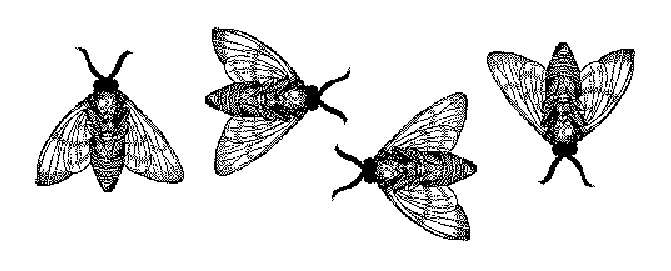
\includegraphics{flies}
\caption{A sample black and white graphic
that needs to span two columns of text.}
\end{figure*}


\begin{figure}
\centering
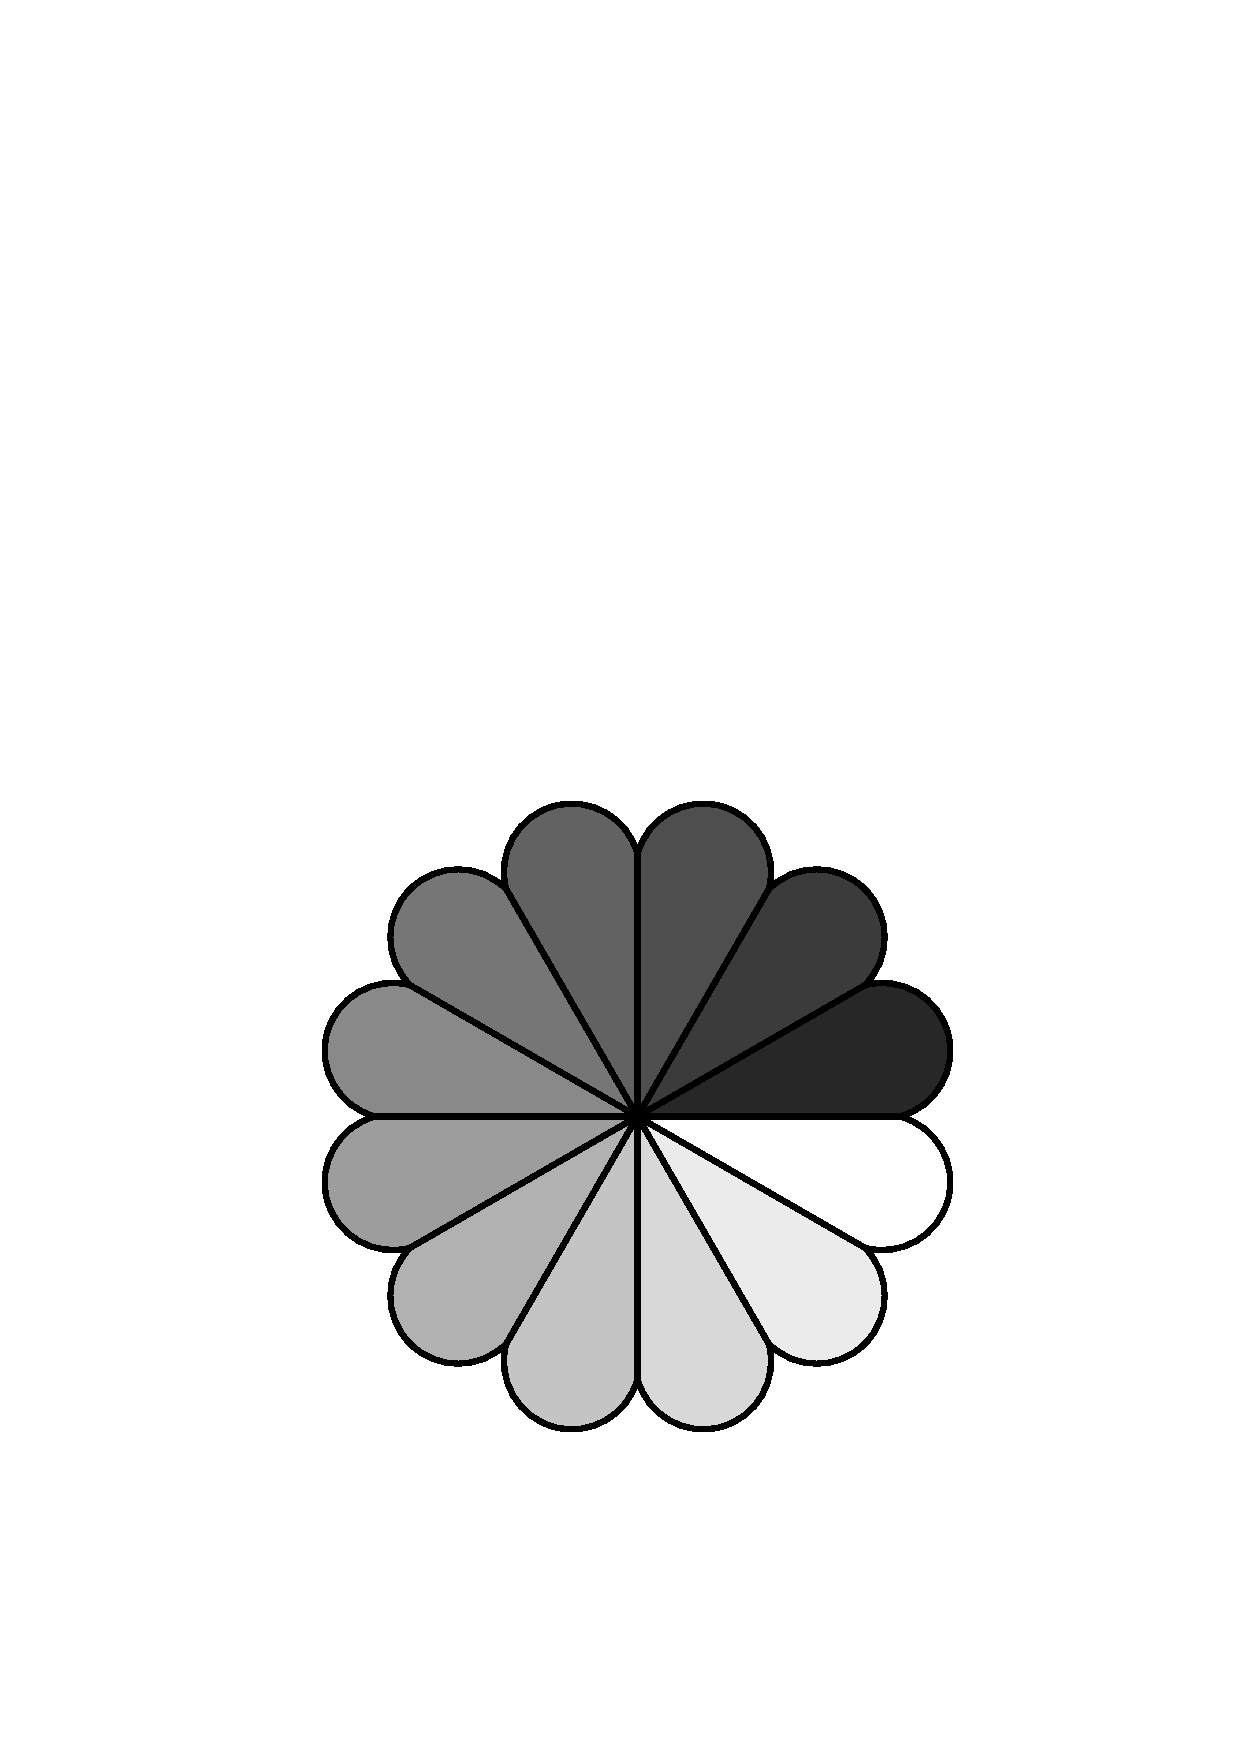
\includegraphics[height=1in, width=1in]{rosette}
\caption{A sample black and white graphic that has
been resized with the \texttt{includegraphics} command.}
\vskip -6pt
\end{figure}

\newtheorem{theorem}{Theorem}
\begin{theorem}
Let $f$ be continuous on $[a,b]$.  If $G$ is
an antiderivative for $f$ on $[a,b]$, then
\begin{displaymath}\int^b_af(t)dt = G(b) - G(a).\end{displaymath}
\end{theorem}

\newdef{definition}{Definition}
\begin{definition}
If $z$ is irrational, then by $e^z$ we mean the
unique number which has
logarithm $z$: \begin{displaymath}{\log e^z = z}\end{displaymath}
\end{definition}

\begin{proof}
Suppose on the contrary there exists a real number $L$ such that
\begin{displaymath}
\lim_{x\rightarrow\infty} \frac{f(x)}{g(x)} = L.
\end{displaymath}
Then
\begin{displaymath}
l=\lim_{x\rightarrow c} f(x)
= \lim_{x\rightarrow c}
\left[ g{x} \cdot \frac{f(x)}{g(x)} \right ]
= \lim_{x\rightarrow c} g(x) \cdot \lim_{x\rightarrow c}
\frac{f(x)}{g(x)} = 0\cdot L = 0,
\end{displaymath}
which contradicts our assumption that $l\neq 0$.
\end{proof}

\end{document}